\documentclass{bioinfo}
\copyrightyear{2005}
\pubyear{2005}

\newcommand{\nb}{\boldsymbol{n}}
\newcommand{\mb}{\boldsymbol{m}}

\begin{document}
\firstpage{1}

\title[Bayesian inference of genetic interactions]{Bayesian inference of genetic interactions}
\author[F\aa berg \textit{et~al}]{Mattias Fr\aa nberg\,$^{1,2,3}$\footnote{to whom correspondence should be addressed}, Bengt Sennblad\,$^{1,2}$, Jens Lagergren\,$^{1,4}$ and Anders Hamsten\,$^2$}
\address{$^{1}$Science for Life Laboratory, Stockholm University, SE-17121, Solna\\
$^{2}$Atherosclerosis Research Unit, Department of Medicine, Karolinska Institutet, SE-171 77, Stockholm,\\
$^{3}$Department of Numerical Analysis and Computer Science, Stockholm University, SE-100 44, Stockholm,\\
$^{4}$School of Computer Science and Communications, KTH Royal Institute of Technology, SE-100 44, Stockholm, Sweden}

\history{Received on XXXXX; revised on XXXXX; accepted on XXXXX}

\editor{Associate Editor: XXXXXXX}

\maketitle

\begin{abstract}

\section{Motivation:}
Text Text Text  Text Text Text Text Text Text Text Text
Text  Text Text Text Text Text Text Text Text Text  Text Text Text Text Text Text Text Text Text  Text Text Text Text Text Text Text Text Text  Text Text Text Text Text Text Text Text Text  Text Text Text Text Text Text Text Text Text  Text Text Text Text Text.

\section{Results:}
Text  Text Text Text Text Text Text Text Text Text  Text Text Text Text Text Text Text Text Text  Text Text Text Text Text Text Text Text Text  Text Text Text Text Text Text

\section{Availability:}
Text  Text Text Text Text Text Text Text Text Text  Text Text Text Text Text Text Text Text Text  Text Text Text Text Text Text Text Text Text  Text

\section{Contact:} \href{mattias.franberg@ki.se}{mattias.franberg@ki.se}
\end{abstract}

\section{Introduction}
Genetic association studies investigates the relationship between genotypes and phenotypes. A natural approach is to search for mutations that are relevant to a heritable disease. Typically you measure this relation for each SNP and perform a statistical test. However, for many diseases this methodology only explain a small proportion of the disease heritability, this phenomena is called the missing heritability. A plausible reason for missing heritability is that SNPs exert a joint effect that is barely visible by looking at single SNPs. For example, if we have two proteins that perform the same function, a loss-of-function mutation in any one of them would not have an effect, only if both of them are mutated at the same time do we see an effect. If we look at the SNPs marginally, we would notice that while the effect only occurs with one of the alleles present, it does not always occur, making it harder to detect the signal. If we however looked at them jointly, we would directly see a clean signal from one combination of alleles. In reality it is not as simple as this but it motivates the development of statistical models that can quantify such effects, the theme of this article.

The problem of inferring genetic interactions is well studied []. But often it is not clear what constitutes a genetic interaction, or joint effect, and how well methods perform compared to each other. The contributions of this paper are:
\begin{itemize}
\item We asses current statistical models for inferring genetic interactions on synthetic data from a set of plausible interaction models.
\item We identify interaction models that are hard to find under the classical ''divergence from additivity'' definition.
\item We propose a novel Bayesian method for inferring genetic interactions. We show that it is coherent with the general intuition of an genetic interaction.
\item We apply our method to the XXX cohort for cardiovascular disease.
\end{itemize}

\section{Approach}
Interactions are hard to formalize. The classical definition "divergence from additivity" is clear from a mathematical perspective, but lacks intuition. In a multiple regression model the cross terms will pick up parts of the function where multiple covariates jointly influence the risk. We say that something interacts if the coefficient for the cross terms are significant. There is nothing unclear from a mathematical point of view, but some questions are raised. For which risk functions do we see an interaction? Can we find all types of interactions or are we restricted?

We define interactions from a probabilistic perspective. Intuitively, an interaction concerns the dependence between random variables. If variables are independent, they are not interacting. We can draw a picture of this dependence structure, as illustrated in figure \ref{fig:01}. Here two variables, or SNPs, each marginally explain a part of the phenotypic uncertainty. Once they are brought together, two things can happen. Firstly, part of what they explain are overlapping, e.g. they could be slightly correlated like SNPs in LD. Secondly, we can have an interaction effect that was not visible when we looked at them marginally, and suddenly they explain more than before. Both of these effects are in some sense interactions, but it is only the second effect that we are interested in. We could write this down as the difference between the joint mutual information minus the marginal mutual information. By looking at these terms we can see that it is just a measure of the divergence of conditional independence.

\begin{figure}[!tpb]%figure1
\centerline{\includegraphics[scale=0.3]{figures/interaction}}
\caption{This figure illustrates the different components of a genetic interaction. The big circles represent the uncertainty of the phenotype. The filled parts of the circle is the uncertainty explained by some part of the model. The upper circles shows the uncertainty explained by two different variables. The bottom circle shows how the explained uncertainty has changed when both variables are included in the model.}\label{fig:01}
\end{figure}

In this paper we measure interaction as the divergence from conditional independence. Mathematically, for any random variables $X_1$, $X_2$ and $Y = g(X_1, X_2)$ where $X$'s represent SNPs and $Y$ a phenotype, and $g$ is any function. We say that an interaction occurs whenever
$$ Pr[ X_1, X_2 \mid Y ] \neq Pr[ X_1 \mid Y ] Pr[ X_2 \mid Y ] $$
This will be true in general so we need to include some measure of significance. In this paper we take a Bayesian approach. There are similar approaches of looking at conditional independence, In [] Moore extend the MDR methodology to test conditional independence, in [] the authors test the difference in mutual information, and in [] conditional independence is tested in the framework of log linear models. All of the methods above are general because they look for any form of relationship. A general method will have less statistical power than a specific method in some situations, because they trade variance for less bias.

\begin{methods}
\section{Methods}
In this section we use the following notation:
\begin{itemize}
\item $f$ represent either a discrete or continuous probability density (discrete probability densities can be treated as continuous densities with a counting measure).
\item $x_1$ and $x_2$ represent to different SNPs. We simplify notation by not indexing individuals.
\item $d$ represent the case/control status.
\item $n_{i,j}$ is the number of controls with genotype $i$ at locus 1 and genotype $j$ at locus 2.
\item $m_{i,j}$ is the number of controls with genotype $i$ at locus 1 and genotype $j$ at locus 2.
\item $n = \sum_{i,j} n_{i,j}$, and $m = \sum_{i,j} m_{i,j}$
\item $L$ is the number of SNP-SNP interactions.
\end{itemize}

X et al. underlined the importance of testing for association while allowing for interaction []. The Bayesian approach to accomplishing this would be to introduce a set of association models, one that allows interaction and one that does not, and then asses the significance by looking at the posterior probability of the interaction model.

Formally we have a set of models
\begin{itemize}
\item $M_u$, the null model without association, models data without association.
\item $M_c$, the conditionally independent model, models association without interaction.
\item $M_f$, the full interaction model, models association with interaction.
\end{itemize}

Let $\mathcal{M} = \{ M_f, M_c, M_u \}$, then the model posterior for the full model becomes
$$ f(M_f \mid D) = \frac{f(D \mid M_f)f(M_f)}{\sum_{M \in \mathcal{M}}f(D \mid M)f(M)}$$
and analogously for the other models. To continue we need to define two things: the model prior $f(M)$ and the actual data models $f(D \mid M)$. The model priors should be formed so that they compensate for multiple tests. We take the approach of [] who treat the problem as a variable selection problem, considering all possible pairs of interactions. We get
\begin{itemize}
\item $f(M_f) = \frac{1}{2^{2L}}$
\item $f(M_c) = \frac{1}{2^{L}}$
\item $f(M_u) = 1 - f(M_f) - f(M_c)$
\end{itemize}
For the data models, we see data as outcomes of a multinomial distribution. The interaction model has two sets of $9$ outcomes, one for cases and one for controls. The conditionally independent model has four sets of $3$ outcomes, and the null model has one set of $9$ outcomes. The densities are factorized as follows:

\begin{eqnarray*}
	f(D \mid M_f)  & = & f( \{ n_{i,j} \} \mid M_f) \cdot f( \{ m_{i,j} \} \mid M_f)\\
	f(D \mid M_c) & = & f( \{ n_{i,\cdot} \} \mid M_c) \cdot f( \{ n_{\cdot, j} \} \mid M_c) \cdot \\
	& & f(\{ m_{i,\cdot} \} \mid M_c) \cdot f( \{ m_{\cdot,j} \} \mid M_c) \\
	f(D \mid M_u) & = & f( \{ n_{i,j} + m_{i,j} \} \mid M_u)
\end{eqnarray*}
As seen above we consider the case/control status to be given, this might appear strange but it is in agreement with how case/control studies are sampled. Since the case/control status of an individual determines whether he or she will be included.

The multinomial parameters are modeled with a Dirichlet prior which is a conjugate prior, meaning that the posterior is also a Dirichlet distribution, and in this case explicit. The $f( \{ n_{i,j} \} \mid M_f)$ is modeled with a Dirichlet with parameters $\alpha_{i,j}= 1$, $f( \{ n_{i,\cdot} \} \mid M_c)$ with $\alpha_i = 1$, and $f( \{ n_{i,j} + m_{i,j} \} \mid M_u)$ with $\alpha_{i,j} = 1$.

We finally get the data probabilities []:
$$ f( \{n_{i,j}\} \mid \{ \alpha_{i,j} \}, M_f) = \frac{ \Gamma \left( A \right) }{ \Gamma\left( n + A \right) } \prod_{i,j} \frac{ \Gamma( n_{i,j} + \alpha_{i,j} ) }{ \Gamma( \alpha_{i,j} ) } $$
where $A = \sum_{i,j} \alpha_{i,j}$, and similarly for the other densities.

\subsection{Logistic regression}
\subsection{Log-linear models}
\end{methods}

\section{Results}

%\begin{figure}[!tpb]%figure1
%%\centerline{\includegraphics{fig01.eps}}
%\caption{Caption, caption.}\label{fig:01}
%\end{figure}
%
%\begin{figure}[!tpb]%figure2
%%\centerline{\includegraphics{fig02.eps}}
%\caption{Caption, caption.}\label{fig:02}
%\end{figure}
%
%\begin{table}[!t]
%\processtable{This is table caption\label{Tab:01}}
%{\begin{tabular}{llll}\toprule
%head1 & head2 & head3 & head4\\\midrule
%row1 & row1 & row1 & row1\\
%row2 & row2 & row2 & row2\\
%row3 & row3 & row3 & row3\\
%row4 & row4 & row4 & row4\\\botrule
%\end{tabular}}{This is a footnote}
%\end{table}

\section{Discussion}

Text Text Text Text Text Text  Text Text Text Text Text Text Text Text Text  Text Text Text Text Text Text. Figure \ref{fig:02} shows that the above method  Text Text Text Text  Text Text Text Text Text Text  Text Text.  \citealp{Boffelli03} might want to know about  text text text text
Text Text Text Text Text Text  Text Text Text Text Text Text Text Text Text  Text Text Text Text Text Text. Figure \ref{fig:02} shows that the above method  Text Text Text Text  Text Text Text Text Text Text  Text Text.  \citealp{Boffelli03} might want to know about  text text text text
Text Text Text Text Text Text  Text Text Text Text.




Table~\ref{Tab:01} shows that Text Text Text Text Text  Text Text Text Text Text Text. Figure \ref{fig:02} shows that
the above method Text Text. Text Text Text  Text Text Text Text Text Text. Figure \ref{fig:02} shows that
the above method Text Text. Text Text Text  Text Text Text Text Text Text. Figure \ref{fig:02} shows that
the above method Text Text.









%%%%%%%%%%%%%%%%%%%%%%%%%%%%%%%%%%%%%%%%%%%%%%%%%%%%%%%%%%%%%%%%%%%%%%%%%%%%%%%%%%%%%
%
%     please remove the " % " symbol from \centerline{\includegraphics{fig01.eps}}
%     as it may ignore the figures.
%
%%%%%%%%%%%%%%%%%%%%%%%%%%%%%%%%%%%%%%%%%%%%%%%%%%%%%%%%%%%%%%%%%%%%%%%%%%%%%%%%%%%%%%






\section{Conclusion}

(Table~\ref{Tab:01}) Text Text Text Text Text Text  Text Text Text Text Text Text Text Text Text  Text Text Text Text Text Text. Figure \ref{fig:02} shows that the above method  Text Text Text Text  Text Text Text Text Text Text  Text Text.  \citealp{Boffelli03} might want to know about  text text text text
Text Text Text Text Text Text  Text Text Text Text Text Text Text Text Text  Text Text Text Text Text Text. Figure \ref{fig:02} shows that the above method  Text Text Text Text  Text Text Text Text Text Text  Text Text.  \citealp{Boffelli03} might want to know about  text text text text
Text Text Text Text Text Text  Text Text Text Text Text Text Text Text Text  Text Text Text Text Text Text. Figure \ref{fig:02} shows that the above method  Text Text Text Text  Text Text Text Text Text Text  Text Text.



Text Text Text Text Text Text  Text Text Text Text Text Text Text Text Text  Text Text Text Text Text Text. Figure \ref{fig:02} shows that the above method  Text Text Text Text  Text Text Text Text Text Text  Text Text.  \citealp{Boffelli03} might want to know about  text text text text





\begin{enumerate}
\item this is item, use enumerate
\item this is item, use enumerate
\item this is item, use enumerate
\end{enumerate}

Text Text Text Text Text Text  Text Text Text Text Text Text Text Text Text  Text Text Text Text Text Text. Figure \ref{fig:02} shows that the above method  Text Text Text Text  Text Text Text Text Text Text  Text Text.  \citealp{Boffelli03} might want to know about  text text text text
Text Text Text Text Text Text  Text Text Text Text Text Text Text Text Text  Text Text Text Text Text Text. Figure \ref{fig:02} shows that the above method  Text Text Text Text  Text Text Text Text Text Text  Text Text.  \citealp{Boffelli03} might want to know about  text text text text
Text Text Text Text Text Text  Text Text Text Text Text Text Text Text Text  Text Text Text Text Text Text.






Text Text Text Text Text Text  Text Text Text Text Text Text Text Text Text  Text Text Text Text Text Text. Figure \ref{fig:02} shows that the above method  Text Text Text Text


\section*{Acknowledgement}
Text Text Text Text Text Text  Text Text.  \citealp{Boffelli03} might want to know about  text text text text

\paragraph{Funding\textcolon} Text Text Text Text Text Text  Text Text.

%\bibliographystyle{natbib}
%\bibliographystyle{achemnat}
%\bibliographystyle{plainnat}
%\bibliographystyle{abbrv}
%\bibliographystyle{bioinformatics}
%
%\bibliographystyle{plain}
%
%\bibliography{Document}


\begin{thebibliography}{}
\bibitem[Bofelli {\it et~al}., 2000]{Boffelli03} Bofelli,F., Name2, Name3 (2003) Article title, {\it Journal Name}, {\bf 199}, 133-154.

\bibitem[Bag {\it et~al}., 2001]{Bag01} Bag,M., Name2, Name3 (2001) Article title, {\it Journal Name}, {\bf 99}, 33-54.

\bibitem[Yoo \textit{et~al}., 2003]{Yoo03}
Yoo,M.S. \textit{et~al}. (2003) Oxidative stress regulated genes
in nigral dopaminergic neurnol cell: correlation with the known
pathology in Parkinson's disease. \textit{Brain Res. Mol. Brain
Res.}, \textbf{110}(Suppl. 1), 76--84.

\bibitem[Lehmann, 1986]{Leh86}
Lehmann,E.L. (1986) Chapter title. \textit{Book Title}. Vol.~1, 2nd edn. Springer-Verlag, New York.

\bibitem[Crenshaw and Jones, 2003]{Cre03}
Crenshaw, B.,III, and Jones, W.B.,Jr (2003) The future of clinical
cancer management: one tumor, one chip. \textit{Bioinformatics},
doi:10.1093/bioinformatics/btn000.

\bibitem[Auhtor \textit{et~al}. (2000)]{Aut00}
Auhtor,A.B. \textit{et~al}. (2000) Chapter title. In Smith, A.C.
(ed.), \textit{Book Title}, 2nd edn. Publisher, Location, Vol. 1, pp.
???--???.

\bibitem[Bardet, 1920]{Bar20}
Bardet, G. (1920) Sur un syndrome d'obesite infantile avec
polydactylie et retinite pigmentaire (contribution a l'etude des
formes cliniques de l'obesite hypophysaire). PhD Thesis, name of
institution, Paris, France.

\end{thebibliography}
\end{document}
